\documentclass[10pt,twocolumn]{article}

\usepackage{myfontstyle}
\usepackage{mypackages}
\usepackage{mymacros}
\usepackage{mycommands}

\begin{document}
\thispagestyle{fancy1}

%%% Title and Abstract------------------------
\twocolumn[
\begin{center}
	\hrule
	\vspace{3pt}
	% Title:
	{\sffamily\bfseries\Large
		Report for Laboratory 03: RC-CIRCUIT RESPONSE
	} \\
	{\color{gray}
		\vspace{3pt}
		\hrule
		\vspace{3pt}
	}
	{
		\hspace*{\fill}
		
		\hspace*{\fill}
		Ryan Haseman
		\hspace*{\fill}
		
		\hspace*{\fill}
%		Fourth Author    % uncomment these two lines if there's a fourth author
%		\hspace*{\fill}
	}\\
	\vspace{3pt}
	{\itshape
		\hspace*{\fill}
		Department of Mechanical Engineering, Saint Martin's University
		\hspace*{\fill} \\
		\hspace*{\fill}
		ME 316---Mechatronics \& Measurements Laboratory
		\hspace*{\fill}
	}\\
	\vspace{3pt}
	{
		\hspace*{\fill}
		\today{} % today's date ... can type manually instead
		\hspace*{\fill}
	}
	\vspace{3pt}
	{\color{gray}\hrule}
%	\vspace{2pt}
\end{center}
% Abstract:
\begin{adjustwidth}{1.5in}{1.5in}
{\small
\noindent\textbf{Abstract.} \hspace{1em}
A RC-circuit was constructed with a 100 k$\Omega$ resistor and 100 $\mu$F capacitor and powered by a 9-volt battery. The voltage across the capacitor was measured using a NI myRIO micro-controller and recorded using LabView as the capacitor charged. The data was then plotted in Matlab for analysis. Using Matlab, a theoretical curve was produced and the exponential nature of a charging capacitor was explored. An analysis was done to investigate and quantify any discrepancy between the theoretical and observed values of the charging capacitor within the circuit. 
}
\end{adjustwidth}
\vspace{9pt}
\hrule
\vspace{1\baselineskip}
]

%%% Body -------------------------

\section{Introduction}

The purpose of this lab was to measure and analyze the time response of a capacitor in a simple RC circuit. The charging of a capacitor in a RC circuit can be modeled as a first order time-invariant dynamic system. A capacitor is an electrical component used to store charge and the time response is the amount of time it takes to become fully charged. As a voltage source was applied to the circuit, a National Instruments (NI) myRIO was used to measure the time response of the capacitor. The data was then compiled in a LabVIEW virtual interface and compared to calculated theoretical values using Matlab.

\begin{figure}[h!]
	\centering
	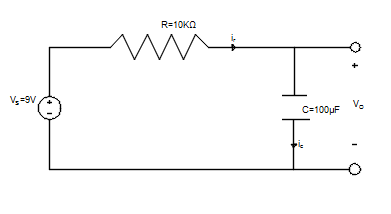
\includegraphics[width=.9\linewidth]{figures/RC.png}
	\caption{RC circuit diagram}
	\label{fig:RC}
\end{figure}

\section{Materials and Methods}

Materials used to perform this lab are listed below:

\begin{itemize}
\item breadboard
\item 9-volt battery
\item 10k$\Omega$ resistor
\item 100$\mu$F capacitor
\item NI myRIO model:1900
\item Fluke 87 V \textit{True RMS Multimeter}
\end{itemize}

A simple RC circuit was built, per \autoref{fig:RC}, for analysis using a standard breadboard. A 9-volt battery was selected as the voltage source along with a capacitor with the nominal capacitance of 100 $\mu$F. The individual components were measured, and connected to the required hardware and software. After computing the resistance required for a time constant of 1 second, a 10k$\Omega$ resistor was selected. The properties of each component in the circuit were then independently measured and recorded and can be found in \autoref{tab:vals}.

\begin{table}[h!]
	\begin{tabularx}{1\linewidth}{ lXX }
		\hline
		 & \textbf{Nominal Value} & \textbf{Measured Value} \\
		\hline
		Resistor & $10\ k \Omega$ & $9.86 \ k \Omega$ \\
		Capacitor & 100\ $\mu$F  & 103\ $\mu$F \\
		Battery & 9 v & $9.15 v$ \\
		\hline
	\end{tabularx}
	\caption{measured values for circuit components}
	\label{tab:vals}
\end{table}

	
	A NI myRIO microprocessor was used for data collection and was connected to a computer running LabView via USB. The NI myRIO was then wired to the breadboard by connecting both AGND (6) and AI0- (8) to the circuit's ground, and connecting AI0+ (7) to the positive capacitor terminal.
	 
	After connecting the hardware, a pre-configured virtual interface (VI) was used to help record data. The VI allowed for the data generated by the NI myRIO to be recorded and displayed graphically. After initiating the data collection VI in LabView, the battery was connected to the circuit, the capacitor was charged, and the voltage across the capacitor was measured and logged at 1 millisecond intervals.  

\section{Results}

\begin{figure}[hbt]
	\centering
	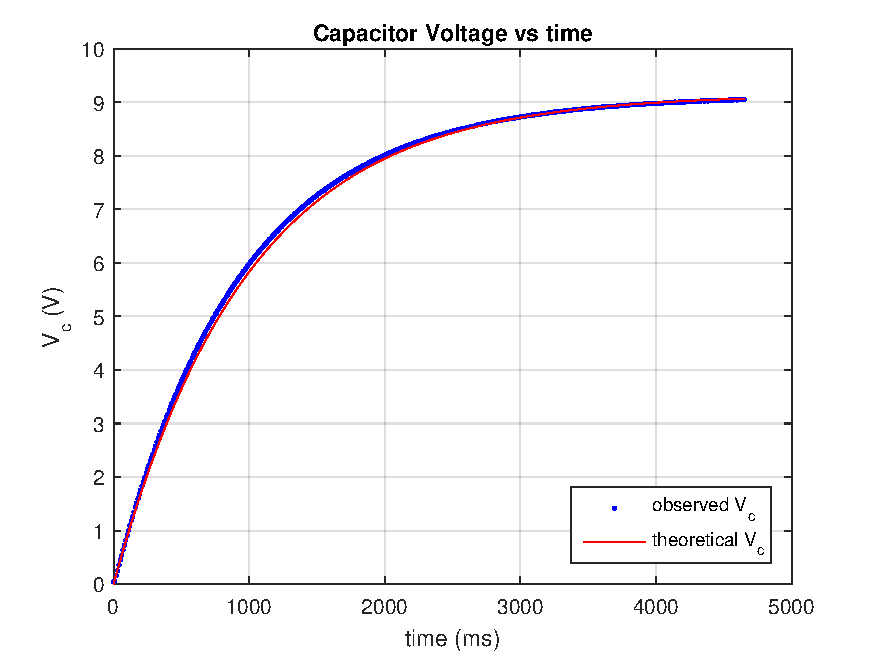
\includegraphics[width=.9\linewidth]{figures/capCharge.pdf}
	\caption{voltage data captured from NI myRIO}
	\label{fig:CapVolt}
\end{figure}

After completing the RC circuit data capture, the NI myRIO collected 1175 data points representing voltage across the capacitor. Plotting these points versus times revealed a tendency for the voltage in the capacitor to rise exponentially towards a horizontal asymptote as time increased. In this case, the horizontal asymptote was the battery voltage (see \autoref{fig:CapVolt}).

	An analytically derived curve was produced using \autoref{eq:final} and was computed in Matlab. The curve was shifted to the right along the abscissa to match the time the circuit was closed during the test. The curve was then superimposed onto the data for comparison.


\section{Discussion}

\begin{figure}[hbt]
	\centering
	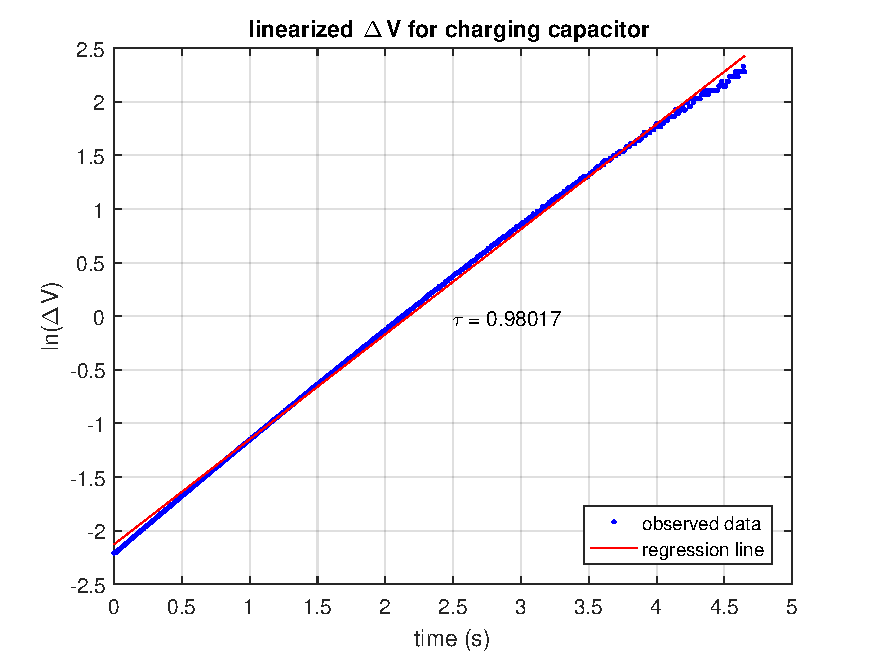
\includegraphics[width=.9\linewidth]{figures/linear.pdf}
	\caption{linearizing the observed data to find $\tau$ }
	\label{fig:lin}
\end{figure}

Using Matlab to take the natural log of the voltage difference between the capacitor and battery supply, the observed data was linearized. A line was fit to it using Matlab's regression polyfit function where order=1. \autoref{fig:lin} was generated to show the linearized data versus the best fit regression line through the data.

From the best fit line in \autoref{fig:lin}, the slope coefficient was determined. This slope, can be interpreted as the time constant ($\tau$) of the charging capacitor in the RC circuit. The observed time constant ($\tau = 0.98\ s$) correlates closely with the calculated constant of $0.99\ s$.  

The linearization of the observed data exasperates the effects of the quantization error of the myRIO A/D converter. The myRIO has a 12-bit LSB A/D converter for the analog inputs used \citep{NI2017}. This correlates to a 4.88mV resolution when converting the analog voltage signal to a digital signal. Any voltage value that is not an integer multiple of 4.88 will be rounded up or down by a maximum of $\pm$ 2.44mV.  This phenomenon can be seen in \autoref{fig:quant} by observing the repeat values of $ln(V_c)$. This effect may be influencing any statistical measures such as the mean error, and standard deviation of the errors.
  
\begin{figure}[hbt]
	\centering
	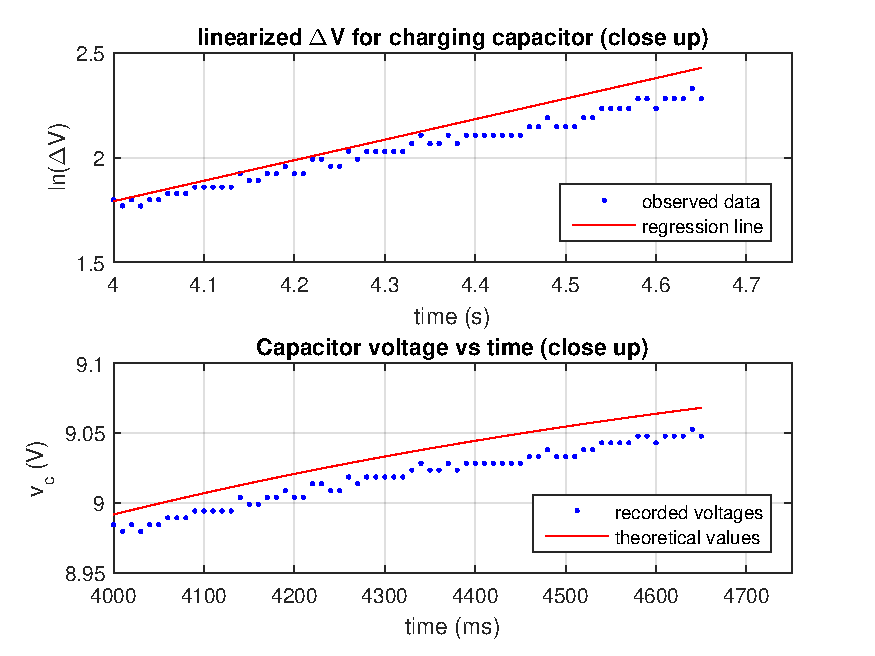
\includegraphics[width=.9\linewidth]{figures/quant.pdf}
	\caption{quantization error observation (shown from 4 - 4.75 seconds) }
	\label{fig:quant}
\end{figure}


\subsection{Error Analysis}

\begin{figure}[hbt]
	\centering
	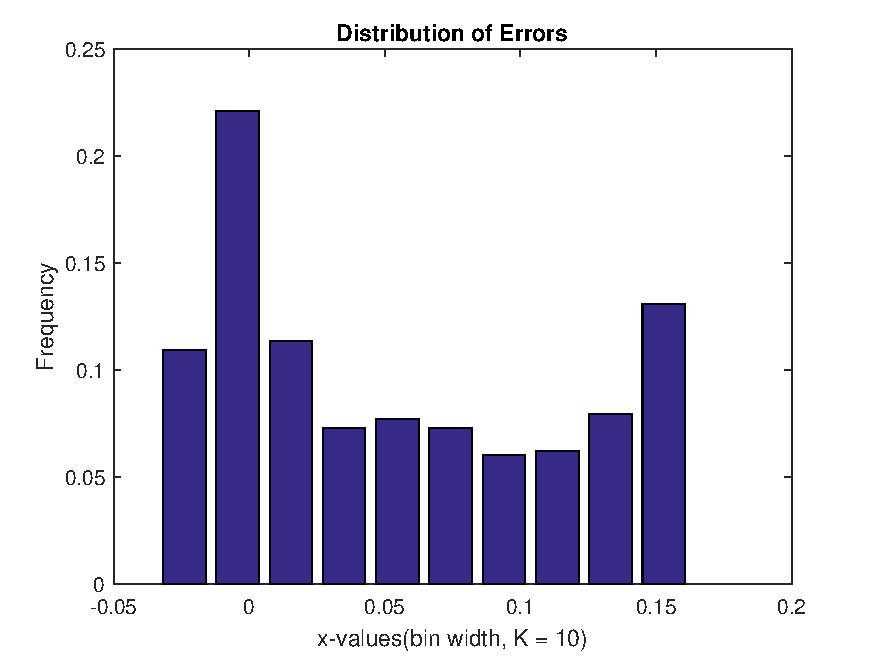
\includegraphics[width=.9\linewidth]{figures/freqDist.pdf}
	\caption{distribution of errors}
	\label{fig:freqD}
\end{figure}

\autoref{fig:freqD} shows a frequency distribution of the difference in the theoretical curve and each data point at time t. The general appearance of this distribution suggests that the error is not normally distributed and cannot be attributed to Gaussian noise.  Most of the error is positive, which highlights the measured response's greater tendency to be over its respective theoretical value. The mean error was calculated to be $54.2$ mV, however the shape of the distribution in \autoref{fig:freqD} suggests that the error distribution may be bimodal, thus having two error means. Further statistical analysis outside the scope of this lab would need to be performed to quantify the error distribution in detail.

\subsection{Uncertainty Analysis}

\begin{table}[h]
	\begin{tabularx}{1\linewidth}{ lXX }
		\hline
		 & \textbf{Accuracy} & \textbf{Uncertainty} \\
		\hline
		Resistor & $0.05\% + 2$ & $5.002\Omega$ \\
		Capacitor & $1\% +5$ & 1.5$\mu$F \\
		Battery & $0.03\%+3$ & $.005$v \\
		\hline
	\end{tabularx}
	\caption{accuracy of Fluke 87V multimeter and corresponding uncertainty of measured components}
	\label{tab:uncert}
\end{table}

From the Fluke 87V \textit{True RMS multimeter} manual \citep{Fluke2017}, the accuracy values for resistance, capacitance and voltage measurements were obtained. \autoref{tab:uncert}, shows the accuracy of each type of measurement as well as the corresponding uncertainty associated with the components measured. This uncertianty value was used to re-plot the capacitor voltage data superimposed with a new theoretical curve bounded by its respective measurement uncertainty as seen in \autoref{fig:bounds}.

\begin{equation} \label{eq:uncert}
\begin{split}
u_{Vc} &= \sqrt{\bigg(\frac{\partial Vc}{\partial R}u_R\bigg)^2 + \bigg(\frac{\partial Vc}{\partial C}u_C \bigg)^2 + \bigg(\frac{\partial Vc}{\partial Vs}u_{Vs} \bigg)^2} \\
Let&\ t = 1\ s\\
And \\
V_c(t) &= V_s(1 - e^{-t/RC})
\end{split}
\end{equation} 

To calculate the overall capacitor voltage uncertainty the sensitivity coefficients were calculated using \autoref{eq:sensitiviy}. 

\begin{equation} \label{eq:sensitiviy}
\begin{split}
\frac{\partial Vc}{\partial Vs} &= 1-e^{-1/RC}\\
\frac{\partial Vc}{\partial R} &= -V_s e^{-1/RC}\frac{1}{CR^2}\\
\frac{\partial Vc}{\partial C} &= -V_s e^{-1/RC}\frac{1}{RC^2}
\end{split}
\end{equation} 

Applying the calculated sensitivity coefficients, along with the uncertainty values found in \autoref{tab:uncert}, an overall measurement uncertainty was found to be $\pm$ 50.6 mV. \autoref{fig:bounds} along with \autoref{fig:freqD} show that the majority of the error lies between the uncertainty bounds and can be contributed to the limitations of the measuring devices.

\begin{equation} \label{eq:uvc}
\begin{split}
u_{Vc} = \pm \ 50.6mV
\end{split}
\end{equation} 

\begin{figure}[hbt]
	\centering
	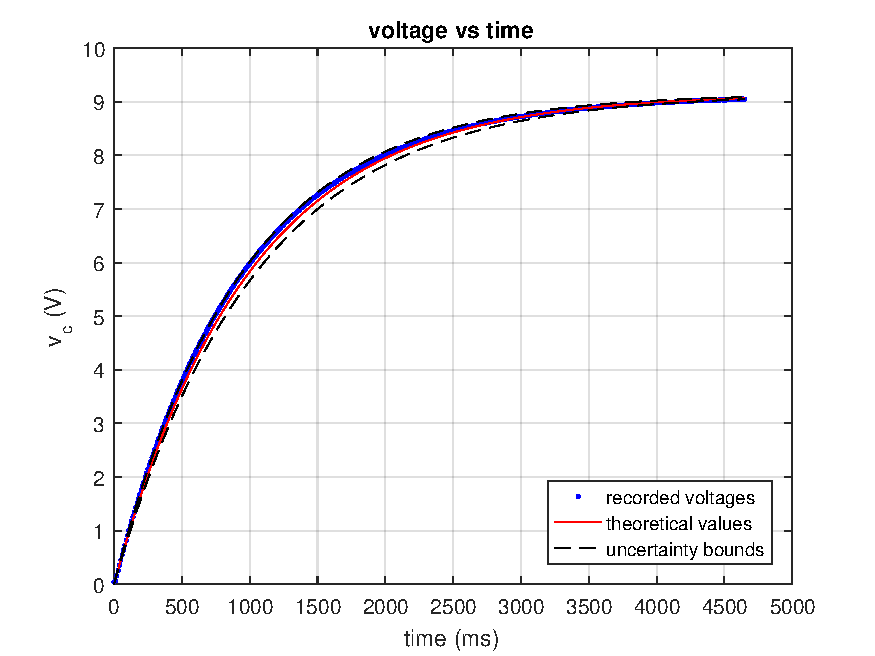
\includegraphics[width=.9\linewidth]{figures/capBounds.pdf}
	\caption{capacitor voltage with bounds}
	\label{fig:bounds}
\end{figure}

A "close-up" plot was generated using data from t = 3 s through t = 4.75 s, to show more detail about the recorded, theoretical and uncertainty bound values.

\begin{figure}[hbt]
	\centering
	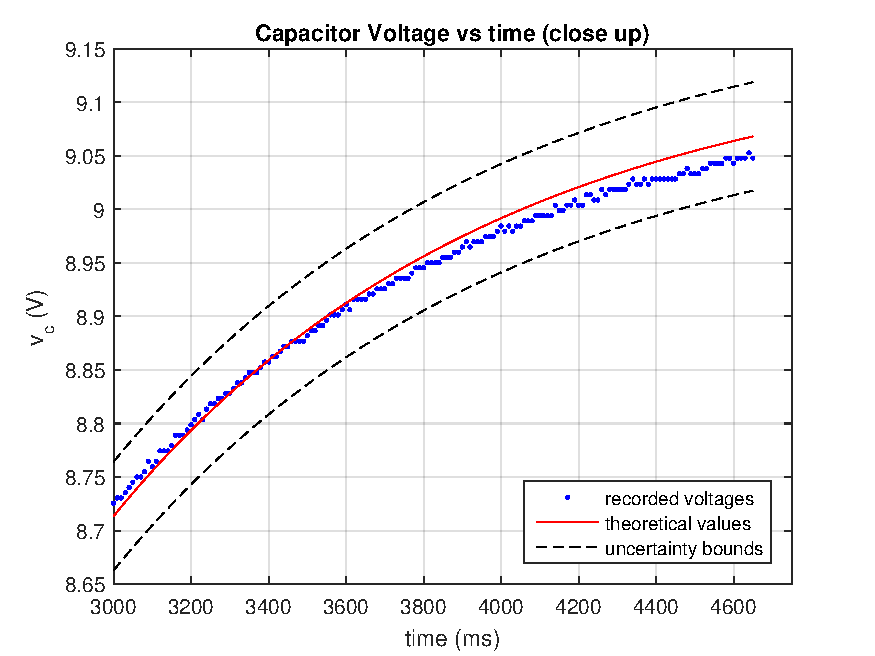
\includegraphics[width=.9\linewidth]{figures/closeUp.pdf}
	\caption{capacitor charging at t = 3-4.75 seconds, with uncertainty bounds}
	\label{fig:bounds}
\end{figure}

\subsection{Conclusion}

Overall, the RC circuit response performed as expected. Although the majority of the observed data was inside the uncertainty bounds of the measurement device, through trial and error, the resistance value was adjusted to fit well within its bounds. The most likely source of error other than measurement uncertainty, was due to human error while taking the measurements of the RC components. To improve on this error, more caution could be taken to secure the multimeter probe connections to the components before a measurement is recorded. 




\appendix

\section{Appendix}

\subsection{Derivation of RC Circuit Response Equation}

Elemental equations for a resistor and a capacitor: 
\begin{equation} \label{eq1}
\begin{split}
V_{R}&=i_{R}R_{1} \\
I&=C\frac{dv}{dt}
\end{split}
\end{equation} 

Kirchhoff's Voltage and Current Law's

\begin{equation} \label{eq2}
\begin{split}
V_{R} + V_{C} - V_{S}&=0 \\
i_{R}&=i_{C}
\end{split}
\end{equation} 


Ordinary Differential Equation:


\begin{equation} \label{eq3}
\begin{split}
%i_{r} & = i_{C}=i \\
%0 & =V_{R}+V_{C}-V_{S} \\
%0 & = i_{R}R+V_{C}-V_{S} \\
%0 & =R(\frac{dv}{dt})+V_{C}-V_{S} \\
%V_{S} & =RC(\frac{dv_c}{dt})+V_{c} \\
RC(\frac{dv_c}{dt})=V_{c}-V_{S} \\
\end{split}
\end{equation}

Using the elemental equations, along with Kirchhoff's Voltage and Current laws, the ODE was derived for the change in voltage with respect to time. With this, the Homogeneous and Particular solutions can be found.


Characteristic Equation: 
\begin{equation} \label{eq4}
\begin{split}
RC\lambda+1&=0 \\
let  \  \tau&=RC\\
\lambda&=\frac{-1}{\tau}
\end{split}
\end{equation} 

Homogeneous and Particular Solution: 
\begin{equation} \label{eq5}
\begin{split}
V_{ch}(t)&=k_{1}e^{-\lambda t}\\
V_{cp}(t)&=k_2\\
\end{split}
\end{equation} 

Plugging the particular solution back into the ODE, the constant (k) can be found: 
\begin{equation} \label{eq6}
\begin{split}
k_2 &=V_{o} \\
V_{o}&= 9.15V
\end{split}
\end{equation}

The general solution for the ODE was found to be:
\begin{equation} \label{eq7}
\begin{split}
V_{c}(t)&=k_{1}e^{-\lambda t} + V_{o}
\end{split}
\end{equation} 

Using the parameters defined by the circuit and an initial condition of $V_{c}(0) = 0$, a specific solution was found for the voltage across the capacitor.

\begin{equation} \label{eq8}
\begin{split}
V_o=9.15V \\
RC = 1 \ s\\
V_{c}(t)=V_{o}(1-e^{-t/RC})\\
\end{split}
\end{equation}

Voltage across the capacitor as a function of time:
\begin{equation} \label{eq:final}
\begin{split}
V_{c}(t)=9.15(1-e^{-t/\tau})
\end{split}
\end{equation}




\bibliographystyle{plainnat}
\bibliography{Lab3}



\end{document}  